\section{Markov chain Monte Carlo (MCMC)}

In this thesis, Markov chains were used to train the presented \acl{sorn}. Before the specific methods are addressed, some theory about Markov chains is introduced.

%%%%% Markov chains %%%%%
\subsection{Markov chains}

\emph{Markov chains} contain a number of states which are changing with a specific probability. The \emph{markov property} states that the probability of the current state only depends on the immediate previous state. Therefore, the Markov property in the discrete case can be defined as follows:

\begin{definition}[Markov property]
Let $(\Omega, \mathcal{F}, \Pb)$ be a probability space and $(S, \mathcal{S})$ a measurable space, where $S = \{x_1, x_2, ... \}$ is a countable set, called state space. A stochastic process $X = \{ X_t : \Omega \to S\}_{t\in\N}$ is said to possess the Markov property if and only if for each $x_0, ..., x_{t+1}\in S$ and $t\in\N$

\begin{equation}
\label{eq:markov-chain}
\Pb(X_{t+1} = x_{t+1} | X_{t} = x_{t}, X_{t-1} = x_{t-1}, ..., X_0 = x_0) = \Pb(X_{t+1} = x_{t+1} | X_{t} = x_{t}).
\end{equation}
\end{definition}

The Markov property is also called \emph{memorylessness}, since it is sufficient to memorize the probability of the state before, no further information is necessary.

The probability of changing from one state to another is called \emph{transition probability}, which is defined as

\begin{equation}
\label{eq:trans-prob}
p_{ij}(t) = \Pb(X_{t+1} = x_j | X_{t} = x_i),
\end{equation}

where $x_i, x_j \in S$ and $i,j \in \N$. The transition probabilities can be summarized in a \emph{transition matrix}. A transition matrix for a finite Markov chain where $i,j \in \{1, ..., n\}$ with $n \in\N$ has the form

\begin{equation}
\label{eq:trans-matrix}
M(t) = (p_{ij}(t))_{i,j \in \{1,...,n\}} = \begin{bmatrix}
p_{11}(t) & p_{12}(t) & \hdots  & p_{1n}(t)\\
p_{21}(t) & \ddots &  & \vdots \\
\vdots &  & \ddots & \vdots \\
p_{n1}(t) & \hdots & \hdots & p_{nn}(t)
\end{bmatrix}.
\end{equation}

\nomenclature{$M$}{Transition matrix of a Markov chain}

% transition graph
% reference to graph from properties

%%%%% Properties %%%%%
\subsection{Properties of Markov chains}
\label{sec:markov-properties}

\begin{figure}
    \centering
    \begin{subfigure}{\textwidth}
    	\centering
        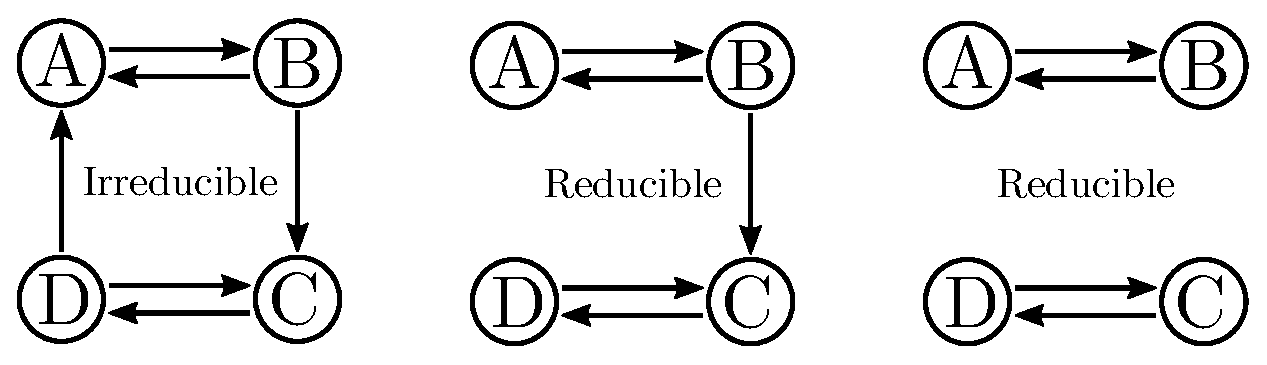
\includegraphics[width=0.7\textwidth]{sorn_markov/mc-irreducible}
        \vspace{5pt}
        \caption{In irreducible Markov chains every state is reachable in finite time, independent of the present state. The first chain on the left side fulfills this property, while the center and right chain do not. The center chain may start in $A$ or $B$, but if $C$ is reached, $A$ and $B$ are not reachable any more. In the right chain, states $A$ and $B$ are totally separated from $C$ and $D$.}
        \vspace{15pt}
        \label{fig:irreducible}
    \end{subfigure}
    \begin{subfigure}{\textwidth}
    	\centering
        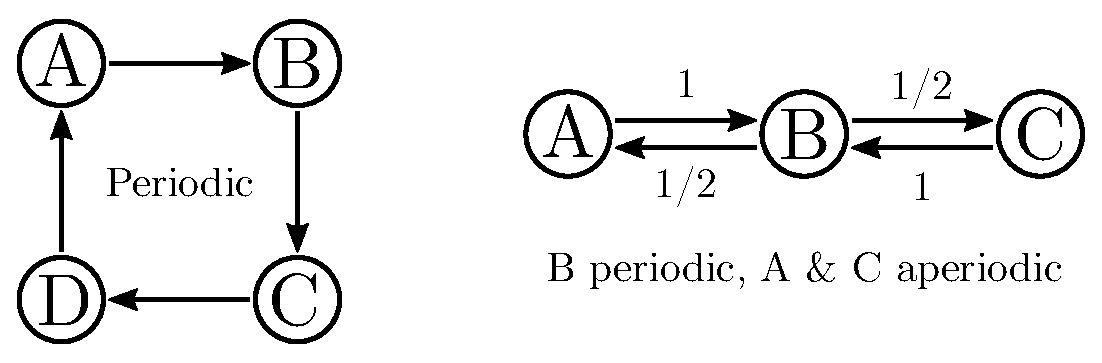
\includegraphics[width=0.7\textwidth]{sorn_markov/mc-aperiodic}
        \vspace{5pt}
        \caption{A state is periodic, if it returns back to the same state periodically, if not, the state is aperiodic. In the chain on the left side every state is periodic, since every state returns after $4$ steps. Therefore, the whole chain is periodic. On the right side, only state $B$ returns periodically every second time, states $A$ and $C$ are not periodic.}
        \vspace{15pt}
        \label{fig:aperiodic}
    \end{subfigure}
    \begin{subfigure}{\textwidth}
    	\centering
        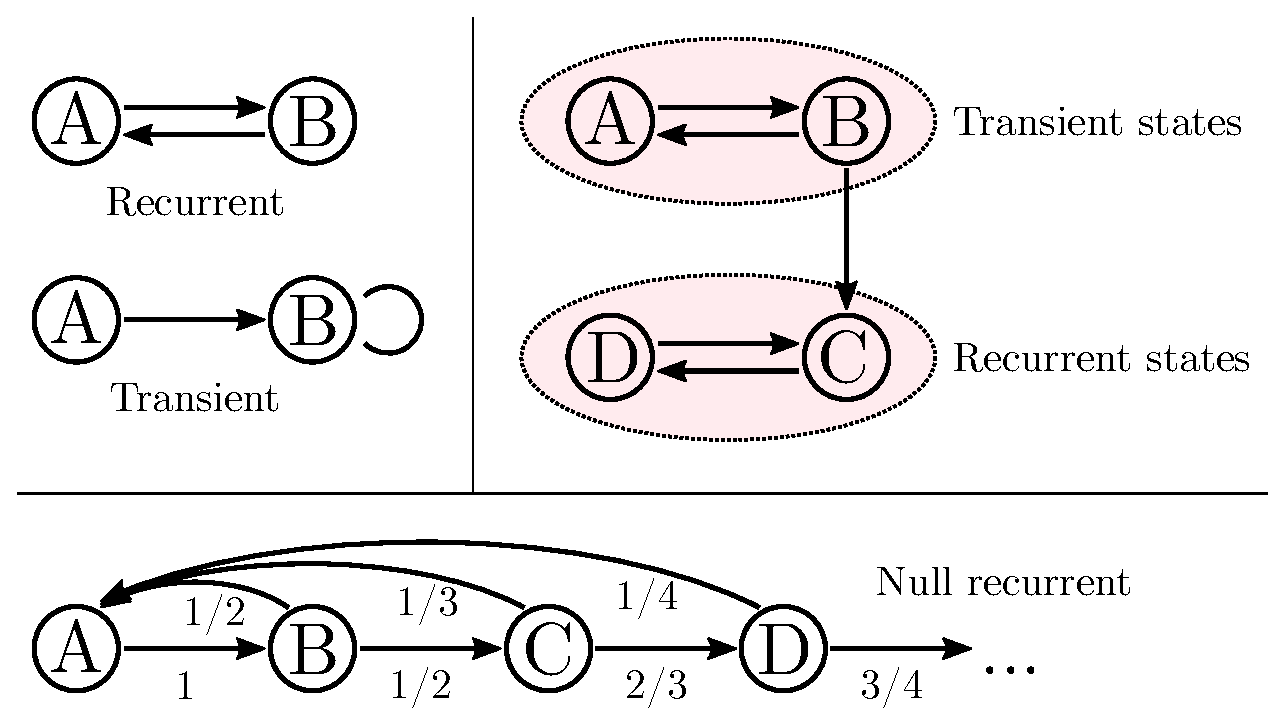
\includegraphics[width=0.7\textwidth]{sorn_markov/mc-recurrent}
        \vspace{5pt}
        \caption{If a state will be reached again almost surely, it is recurrent, otherwise transient. Two simple examples are given on top left. In the first small chain, both states $A$ and $B$ will be reached again all the time. In the second example $A$ directly goes to $B$ and will not be active any more. State $A$ is transient. On the top right, states $A$ and $B$ are transient. If $C$ is activated the first time, the chain will never reach $A$ and $B$ again. On the other hand, $C$ and $D$ are recurrent, both can be reached again all the time. The last example on the bottom shows a null recurrent case. Shown is a Markov chain with infinite states. Since the probability of going back to $A$ is decreasing with a sequence $1/n$ for $n \to\infty$, the time to go back to $A$ is $\E[T_A] = \infty$. Regarding the last chain, more details can be found in a proof in appendix in section \ref{sec:proof-null-recurrent}.}
        \label{fig:recurrent}
    \end{subfigure}
    \caption[Markov chain properties]{Three properties of Markov chains are shown: irreducibility, periodicity and recurrence. If no probability is written at an arrow, the probability is simply $p > 0$.}
    \label{fig:mc-properties}
\end{figure}

\paragraph{a) Homogeneous / Stationary Markov chain}

If the transition probabilities $p_{ij}(t)$ from state $x_i$ to state $x_j$ are independent from time $t$, i.e. $p_{ij}(t) = p_{ij}$ for all $t\in\N$, the Markov chain is called \emph{homogeneous} or stationary Markov chain. It means that

\begin{equation}
\label{eq:markov-homo}
p_{ij} = \Pb(X_{t+1} = x_j | X_t = x_i) =  \Pb(X_t = x_j | X_{t-1} = x_i).
\end{equation}

\paragraph{b) Irreducible Markov chain}

In \emph{irreducible} Markov chains, any state is reachable in finite time, independent of the present state. Formally a Markov chain is irreducible if there exists any $m < \infty$ with

\begin{equation}
\Pb(X_{t+m} = x_j | X_t = x_i) = p_{ij}^{(t+m)} > 0
\end{equation}

for all $i,j$. Examples for reducible and irreducible Markov chains are given in figure \ref{fig:irreducible}.

\paragraph{c) Aperiodic Markov chain}

If a state $x_i$ returns with a multiple of $k$ again to state $x_i$, it is called \emph{periodic}, otherwise \emph{aperiodic}. Formally a \emph{period} is defined as

\begin{equation}
k = \text{gcd} \{ t > 0\,:\,\Pb(X_t = x_i | X_0 = x_i) = p_{ii}^{(t)} > 0 \},
\end{equation}

where $\text{gcd}$ is the greatest common divisor. If the set is empty, the period is not defined. In case that $k=1$ the state $x_i$ is aperiodic and otherwise, if $k>1$, $x_i$ is periodic.

If all states are aperiodic, the Markov chain is called aperiodic. Examples for periodicity and aperiodicity are given in figure \ref{fig:aperiodic}.

\paragraph{d) Recurrent Markov chain}

A state $x_i$ of a Markov chain is called \emph{recurrent} if it  will be reached again almost surely. Therefore, the probability to come back to state $x_i$ is one. Let

\begin{equation}
\label{eq:first-comeback}
T_{x_i} = \inf\{ t \ge 0 \,:\, X_t = x_i | X_0 = x_i \}
\end{equation}

\nomenclature{$T_{x_i}$}{Number of steps until a Markov state is reached again for the first time}

be a random variable, which defines the number of steps until state $x_i$ is reached again for the first time and let $\Pb(T_{x_i} = t)$ the probability to reach $x_i$ again for the first time after exactly $t$ steps. Then state $x_i$ is recurrent, if and only if

\begin{equation}
\label{eq:recurrent}
\Pb(T_{x_i} < \infty) = \sum_{t=1}^\infty \Pb(T_{x_i} = t) = 1,
\end{equation}

If a state is not recurrent, it is called \emph{transient}, which is the case if $\Pb(T_{x_i} < \infty) < 1$. It means that the state will not be reached again almost surely.

Furthermore, if the state is recurrent and the expected value is finite, thus

\begin{equation}
\label{eq:first-comeback-expect}
\E[T_{x_i}] = \sum_{t=1}^\infty t \cdot \Pb(T_{x_i} = t) < \infty,
\end{equation}

the state is called \emph{positive recurrent}. Otherwise, if $\E[T_{x_i}] = \infty$, it is called \emph{null recurrent}.

If all states are (positive) recurrent, the Markov chain is called (positive) recurrent. Examples for recurrent and transient Markov chains are given in figure \ref{fig:recurrent}. A proof for the null recurrent chain in the figure can be found in the appendix in section \ref{sec:proof-null-recurrent}.

%%%%% Stationary %%%%%
\subsection{Stationary distribution}
\label{sec:stat-markov}

%* Definition of stationary distribution\\ 
%* Theorems about stationary distribution

\begin{definition}[Stationary distribution]

Given a homogeneous Markov chain in discrete time $t \in \N$ on state space $S = \{x_1, x_2, ...\}$, the distribution $\Pb_\pi$ is called stationary distribution if and only if

\begin{equation}
\label{eq:markov-stat}
\bm\pi_{x_j} = \Pb_\pi(X_t = x_j) = \sum_{x_i \in S} \Pb_\pi(X_t = x_i)\,p_{ij} \overset{\eqref{eq:markov-homo}}{=} \sum_{x_i \in S} \Pb_\pi(X_t = x_i)\,\Pb(X_t = x_j | X_{t-1} = x_i)
\end{equation}

for all $x_j \in S$.
\end{definition}

\nomenclature{$\bm\pi$}{Stationary distribution of a Markov chain}

The stationary distribution should not be confused with the stationary Markov chain. While the stationary Markov chain is stationary regarding the transition probabilities, the stationary distribution is stationary regarding the probability of the states. Furthermore, the presence of a stationary Markov chain (homogeneous Markov chain) is a condition for the existence of a stationary distribution.

It is not always given that a stationary distribution exists. Furthermore a stationary distribution is not necessarily unique. In the following, first, the general Perron-Frobenius-Theorem \parencite{seneta2006non, pillai2005perron} is presented. Based on this theorem, a statement about the stationary distribution can be derived. While this theorem is highly useful, it assumes aperiodic Markov chains, which are not given in any case. Hence, afterwards another theorem is introduced, which lowers the assumption. At that point I want to remind, that a \emph{homogeneous} Markov chain is assumed in the following.

\begin{definition}[Primitive matrix]
Given a squared matrix $Q = (q_{ij})_{i,j \in\N}$, it is called a primitive matrix if all items are non-negative, $q_{ij} > 0 \,\forall i,j$, denoted by $Q > 0$ and if a $k \in \N$ exists, such that all items of the matrix $Q^k$ ($k$-th power of $Q$) are positive, denoted by $Q^k > 0$.
\end{definition}

\begin{theorem}[Perron-Frobenius]
\label{eq:perron-frobenius}
Suppose $Q$ is an $n \times n$ non-negative primitive matrix. Then there exists an eigenvalue $r$, called Perron-Frobenius eigenvalue, such that:

\begin{enumerate}
\item $r$ is real and positive, $r>0$.
\item $r$ can be associated with strictly positive left and right eigenvectors.
\item $r > |\lambda|$ for any other eigenvalue $\lambda \neq r$.
\item The eigenvectors associated with $r$ are unique to constant multiples.
\item If $0 \le B \le Q$ and $\beta$ is eigenvalue of $B$, then $|\beta| \le r$. Moreover, $|\beta| = r$ implies $B = Q$.
\item $r$ is a simple root of the characteristic equation of $Q$.
\end{enumerate}
\end{theorem}

A proof is given in \textcite[Theorem 1.1]{seneta2006non}. Using the Perron-Frobenius theorem it is possible to state in which cases a unique solution for the stationary distribution can be found.

\begin{theorem}
\label{th:markov-stat}
Let $M$ be a transition matrix and $\bm 1$ a vector where all entries are one. An irreducible and aperiodic Markov chain has a unique stationary distribution given by the solution $\bm\pi$ of $\bm\pi^T M = \bm\pi^T$, where $\bm\pi^T \mathbf{1} = 1$.
\end{theorem}

This theorem will be proven, but two corollaries are necessary.

\begin{corollary}
\label{co:primitive}
An irreducible and aperiodic matrix is primitive.
\end{corollary}

\begin{corollary}
\label{co:smallest-largest}
Let $Q$ be a positive square matrix. Then the minimal row sum is a lower bound and the maximal row sum is an upper bound of the the largest eigenvalue of $Q$.
\end{corollary}

\begin{proof}[Proof for theorem \ref{th:markov-stat}]
Since any transition matrix $M$ is per definition square and non-negative, the statements of the Perron-Frobenius theorem hold for transition matrix $M$, if the Markov chain is primitive. Since corollary \ref{co:primitive} states that any irreducible and aperiodic matrix is primitive, the assumptions of the theorem are clarified.

Furthermore, it holds that

\begin{equation*}
M\mathbf{1} = \mathbf{1},
\end{equation*}

since every row sums to one by definition of the transition matrix. Hence, $M$ has an eigenvalue of $1$ and an eigenvector of $\mathbf{1}$. With corollary \ref{co:smallest-largest}, the largest eigenvalue is exactly the row sum $1$, since all rows of $M$ have the same sum. Therefore, the eigenvalue $r=1$ is the Perron-Frobenius eigenvalue, since property (3) of the theorem states that all other eigenvalues are smaller in absolute. The corresponding right Perron-Frobenius eigenvector is $\mathbf{1}$.

Assuming that a vector $\bm v^T$ is normed, such that $\bm v^T \mathbf{1} = 1$, the eigenvalue problem for the left eigenvector $\bm v^T$ has the following form:

\begin{equation*}
\bm v^T M = r \bm v^T = \bm v^T
\end{equation*}

From statement (2), we know that the left eigenvector regarding $r$ is strictly positive. Therefore, $\bm v^T = \bm\pi^T$ is a distribution, the stationary distribution.

Finally, statement (4) of the Perron-Frobenius theorem states that $\bm\pi$ is unique.
\end{proof}

As a side note, using theorem \ref{th:markov-stat}, the stationary distribution can be calculated as a right eigenvalue problem, just by transposing both sides $(\bm\pi^T M)^T = (\bm\pi^T)^T$, which results in $M^T \bm\pi = \bm\pi$.

Theorem \ref{th:markov-stat} is limited to aperiodic Markov chains. Another theorem lowers the assumptions.

\begin{theorem}
\label{th:irr-rec}
An irreducible and positive recurrent Markov chain has a unique stationary distribution $\bm\pi$ given by

\begin{equation}
\pi_{x_i} = \frac{1}{\E[T_{x_i}]}
\end{equation}
\end{theorem}

A proof is given in \textcite[Corollary 1.2.29]{bladt2017matrix}. The theorem uses the definition of the random variable $T_{x_i}$ from equation \eqref{eq:first-comeback}, which indicates the number of steps, necessary to come back to state $x_i$ again for the first time. Furthermore $\E[T_{x_i}]$ was defined in equation \eqref{eq:first-comeback-expect}.

\begin{theorem}
An irreducible and finite Markov chain is positive recurrent.
\end{theorem}

This theorem is proven in \textcite[Theorem 3.3]{bremaud2013markov}. It shows, that theorem \ref{th:irr-rec} is highly practical for finite Markov chains. Since, in case of finite Markov chains, only the property of irreducibility needs to be fulfilled.

The Perron-Frobenius theorem has a slight advantage, compared to theorem \ref{th:irr-rec}. Using the Perron-Frobenius theorem, it can be shown that even a \emph{limiting distribution} can be obtained. It is defined by $\pi_i = \lim_{t \to\infty} \Pb(X_t = x_i)$. In case of theorem \ref{th:irr-rec}, this is not necessarily the case. If we assume for example a periodic Markov chain with just two states, which are alternating $(0,1,0,1,0,1, ...)$, the Markov chain has no limiting distribution, but a unique stationary distribution. However, for calculating stationary distributions, in most cases theorem \ref{th:markov-stat} was used.

%%%%% Measures %%%%%
\subsection{Measures}
\label{sec:markov-measures}

To evaluate the stationary distribution many measures can be used, which are common for any distribution, not only for Markov chains. Two types are introduced, which are used in the results. At first, information measures, namely variance and Kullback-Leibler divergence, are defined and afterwards a measure for the concentration of a distribution is presented, where the Lorenz curve and the Gini coefficient are introduced. Note that the Gini coefficient is directly derived from the Lorenz curve.

\paragraph{Information measures}

For simplification, the state space can be defined as $S = \{1, ..., n\}$ where $n \in\N$. A simple measure for the stationary distribution is the deviation of the probabilities from their mean probability. Therefore an empirical variance measure is used by calculating

\begin{equation}
\label{eq:variance-estimate}
\sigma^2_\pi = \frac{1}{n} \sum_{k=1}^n (\pi_k - \bar\pi)^2,
\end{equation}

where $\bar\pi = \frac{1}{n} \sum_{k=1}^n \pi_k$. In the following it is just called \emph{variance}.

% If $\Pi = (\Pi_1, ..., \Pi_n)^T$ denotes a random variable for the stationary distribution, the variance of the stationary distribution is given by

% \begin{equation}
% \label{eq:variance}
% \Var(\Pi) = \E[(\Pi - \E[\Pi])^T (\Pi - \E[\Pi])],
% \end{equation}

% which can be interpreted as the expected squared distances between the probabilities of the stationary distribution and their expectation value.

% Since the random variable $\Pi$ depends on the stochastic transition matrix, with probabilities $\Pb(X_{t+1} = x_i | X_t = x_j)$, where $X_t$ is the random variable of the current state at time $t$, it is not easy to obtain the variance analytically. Therefore, a simple estimator is suggested, defined by

% \begin{equation}
% \label{eq:variance-estimate}
% \widehat{\Var(\Pi)} = \sigma^2_\pi = \sum_{k=1}^n (\pi_k - \bar\pi)^2,
% \end{equation}

% where $\bar\pi = \frac{1}{n} \sum_{k=1}^n \pi_k$.

Another measure uses the Kullback-Leibler divergence. If $\bm\pi' \in \{\pi'_1, ..., \pi'_n\} = \{1/n, ..., 1/n\}$ is a stationary distribution where all states are equally probable, the Kullback-Leibler divergence can be obtained by

\begin{equation}
\label{eq:kullbackleibler}
\DKL = \sum_{i=1}^n \pi_i \ln{\left(\frac{\pi_i}{\pi'_i}\right)}.
\end{equation}

The Kullback-Leibler divergence can be understood as relative entropy. It describes the increase in information which is necessary to describe $\bm\pi$, when $\bm\pi'$ is given. It is important to note that the Kullback-Leibler divergence is an asymmetric measure. The value of the measure depends on the order of the distributions and therefore the divergence does not fulfill the properties of a \emph{metric}. It is in particular different from the \emph{total variation distance} $\delta(\bm\pi, \bm\pi')$. A link between the total variation distance and the Kullback-Leibler divergence is given by \emph{Pinsker's inequality}. However, \emph{Gibb's inequality} states that

\begin{equation}
\label{eq:kullbackleibler-gibbs}
\DKL \ge 0
\end{equation}

and $\DKL = 0$ if and only if $\bm\pi = \bm\pi'$, which means that a divergence of $0$ indicates a match between the distributions $\bm\pi$ and $\bm\pi'$.

\begin{SCfigure}[0.6][!b]
    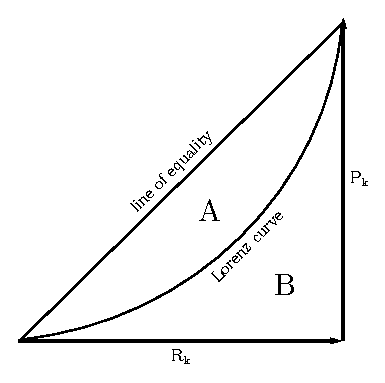
\includegraphics[width=0.45\textwidth]{sorn_markov/lorenz}
    \caption[Lorenz curve]{Illustration of a Lorenz curve. On the $x$-axis is the cumulative share of the probabilities from the states of an equally distributed stationary distribution. On the $y$-axis is the cumulative share of the probabilities of the actual stationary distribution. If the actual distribution is equally distributed, the Lorenz curve reaches the line of equality. The Gini coefficient is calculated by $G = A / (A+B)$.}
    \label{fig:lorenz-illustration}
\end{SCfigure}

\paragraph{Concentration measures}

Another way of evaluating the properties of a Markov chain is to plot the \emph{Lorenz curve} and calculate the \emph{Gini coefficient}. Traditionally, both is often applied to indicate inequality regarding income, used in social sciences. But the Lorenz curve shows the concentration of a distribution in general, whereas the Gini coefficient is a related measure for the intensity of the concentration of the given distribution.

First, assume that $\bm\pi = (\pi_1, ..., \pi_n)^T$ is sorted in a sense that $\pi_1 \le ... \le \pi_n$ and denote $r_i = 1/n$ as the share of a state with probability $\pi_i$, where $n\in\N$ is the number of states. Furthermore $R_k = \sum_{i=1}^k r_i = \sum_{i=1}^k 1/n = k/n$ is the cumulative share of the states. On the other hand, $P_k = \sum_{i=1}^k \pi_i$ is the cumulated probability of $\bm\pi$. The \emph{Lorenz curve} shows the cumulated share of states $R_k$ at the $x$-axis and the cumulated probability $P_k$ at the $y$-axis. If all probabilities are equal, it will result in a straight diagonal line. The more the distribution $\bm\pi$ is concentrated, the more the line will appear in the right bottom corner. An illustration is given in figure \ref{fig:lorenz-illustration}.

Finally, the \emph{Gini coefficient} $G$ is the ratio of the area that lies between the diagonal line, where all states are equal probable, and the area between the actual Lorenz curve and the diagonal. The more the Lorenz curve tends to the corner and, therefore, the more the stationary distribution is unequal, the more the Gini coefficient will tend to $1$, where $1$ represents a perfect concentrated situation. It means that the whole probability is concentrated at one state, the other states are zero. If the distribution is perfectly equal, the Gini coefficient will reach $0$. It can be shown that $G \in [0,1]$ is half of the \emph{relative mean absolute difference}. Hence, for the discrete case, the Gini coefficient is defined as

\begin{equation}
\label{eq:gini}
G = \frac{\sum_{i=1}^n \sum_{j=1}^n |\pi_i - \pi_j|}{2n\cdot \sum_{i=1}^n \pi_i}.
\end{equation}

%%%%% Monte Carlo %%%%%
\subsection{Markov Chain Monte Carlo (MCMC)}

A \emph{Monte Carlo simulation} is a stochastic procedure where random samples are drawn many times. As a result, numerical solutions for analytically difficult or even impossible problems are obtained. \textcite{thomopoulos2012essentials} described the process as follows:

\begin{quote}
To apply the Monte Carlo method, the analyst constructs a mathematical model that simulates a real system. A large number of random sampling of the model is applied yielding a large number of random samples of output results from the model.
\end{quote}

Specifically, if random samples are drawn from the distribution of a Markov chain, it is called \acfi{mcmc} method which includes a broad class of algorithms. Famous and well known algorithms are the \emph{Metropolis–Hastings algorithm} \parencite{hastings1970monte} or the \emph{Gibbs sampler} \parencite{geman1984stochastic}. These techniques are often used in Bayesian inference to evaluate posterior distributions.

There are many different possibilities to understand the behavior of neural networks under the perspective of \acs{mcmc} sampling. For example, there are applications for Boltzmann machines \parencite{osogami2017boltzmann} or energy-based models in general \parencite{goodfellow2007deep}. In \acs{sorn}, it is possible to view the learned time-dependent input patterns under the perspective of \acs{mcmc} sampling. The approach will be introduced in methods (section \ref{sec:methods}) and many illustrative implementations will be given in results (section \ref{sec:results}).

%%%%% MCMC / ANN %%%%%
%\subsection{MCMC and neural networks}

%An overview to MCMC methods in neural networks is given in \cite{andrieu2003introduction}.

%Boltzmann machines, which are a special kind of a stochastic recurrent neural networks, highly depend on a MCMC approach. They are trained by stochastic gradient, where expected values need to be calculated. In many cases those expected values cannot be calculated analytically. Therefore MCMC methods, especially Gibbs sampling can be used to finally train Boltzmann machines \parencite{osogami2017boltzmann}. The MCMC approach can also be used for the broader class of energy-based models \parencite{goodfellow2007deep}.

%MCMC can also be used for model selection. It can for example applied to estimate the number of neurons in a network (3 citations).
% http://www.cs.ubc.ca/~arnaud/andrieu_defreitas_doucet_jordan_intromontecarlomachinelearning.pdf (Seite 23)

%Sampling Maas / Sampling perspective

%It can be summarized that MCMC plays an important role in specific applications of neural networks. The last application should be kept in mind, since in methods section another perspective is introduced, which is inspired by the approach of (paper Maas).

%Where was it used in literature before? link to neural networks?

%Introduce perspective to SORN networks -> In methods



















